\documentclass{sigchi}

% Use this section to set the ACM copyright statement (e.g. for
% preprints).  Consult the conference website for the camera-ready
% copyright statement.

% Copyright
\CopyrightYear{2020}
%\setcopyright{acmcopyright}
\setcopyright{acmlicensed}
%\setcopyright{rightsretained}
%\setcopyright{usgov}
%\setcopyright{usgovmixed}
%\setcopyright{cagov}
%\setcopyright{cagovmixed}
% DOI
\doi{https://doi.org/10.1145/3313831.XXXXXXX}
% ISBN
\isbn{978-1-4503-6708-0/20/04}
%Conference
\conferenceinfo{Asian CHI Symposium '20,}{April  25--30, 2020, Honolulu, HI, USA}
%Price
\acmPrice{\$15.00}

% Use this command to override the default ACM copyright statement
% (e.g. for preprints).  Consult the conference website for the
% camera-ready copyright statement.

%% HOW TO OVERRIDE THE DEFAULT COPYRIGHT STRIP --
%% Please note you need to make sure the copy for your specific
%% license is used here!
% \toappear{
% Permission to make digital or hard copies of all or part of this work
% for personal or classroom use is granted without fee provided that
% copies are not made or distributed for profit or commercial advantage
% and that copies bear this notice and the full citation on the first
% page. Copyrights for components of this work owned by others than ACM
% must be honored. Abstracting with credit is permitted. To copy
% otherwise, or republish, to post on servers or to redistribute to
% lists, requires prior specific permission and/or a fee. Request
% permissions from \href{mailto:Permissions@acm.org}{Permissions@acm.org}. \\
% \emph{CHI '16},  May 07--12, 2016, San Jose, CA, USA \\
% ACM xxx-x-xxxx-xxxx-x/xx/xx\ldots \$15.00 \\
% DOI: \url{http://dx.doi.org/xx.xxxx/xxxxxxx.xxxxxxx}
% }

% Arabic page numbers for submission.  Remove this line to eliminate
% page numbers for the camera ready copy
% \pagenumbering{arabic}

% Load basic packages
\usepackage{balance}       % to better equalize the last page
\usepackage{graphics}      % for EPS, load graphicx instead 
\usepackage[T1]{fontenc}   % for umlauts and other diaeresis
\usepackage{txfonts}
\usepackage{mathptmx}
\usepackage[pdflang={en-US},pdftex]{hyperref}
\usepackage{color}
\usepackage{booktabs}
\usepackage{textcomp}

% Some optional stuff you might like/need.
\usepackage{microtype}        % Improved Tracking and Kerning
% \usepackage[all]{hypcap}    % Fixes bug in hyperref caption linking
\usepackage{ccicons}          % Cite your images correctly!
% \usepackage[utf8]{inputenc} % for a UTF8 editor only

% If you want to use todo notes, marginpars etc. during creation of
% your draft document, you have to enable the "chi_draft" option for
% the document class. To do this, change the very first line to:
% "\documentclass[chi_draft]{sigchi}". You can then place todo notes
% by using the "\todo{...}"  command. Make sure to disable the draft
% option again before submitting your final document.
\usepackage{todonotes}

% Paper metadata (use plain text, for PDF inclusion and later
% re-using, if desired).  Use \emtpyauthor when submitting for review
% so you remain anonymous.
\def\plaintitle{Grit: A Novice Programmer Support Tool for DevOps Integration}
\def\plainauthor{Tyrone Justin Sta Maria, Gavin Raine Dizon, Vince Anthony Esquivel, Jordan Aiko Deja and Unisse Chua}
\def\emptyauthor{}
\def\plainkeywords{devops; novice programmers; programmer support}
\def\plaingeneralterms{Programming}

% llt: Define a global style for URLs, rather that the default one
\makeatletter
\def\url@leostyle{%
  \@ifundefined{selectfont}{
    \def\UrlFont{\sf}
  }{
    \def\UrlFont{\small\bf\ttfamily}
  }}
\makeatother
\urlstyle{leo}

% To make various LaTeX processors do the right thing with page size.
\def\pprw{8.5in}
\def\pprh{11in}
\special{papersize=\pprw,\pprh}
\setlength{\paperwidth}{\pprw}
\setlength{\paperheight}{\pprh}
\setlength{\pdfpagewidth}{\pprw}
\setlength{\pdfpageheight}{\pprh}

% Make sure hyperref comes last of your loaded packages, to give it a
% fighting chance of not being over-written, since its job is to
% redefine many LaTeX commands.
\definecolor{linkColor}{RGB}{6,125,233}
\hypersetup{%
  pdftitle={\plaintitle},
% Use \plainauthor for final version.
%  pdfauthor={\plainauthor},
  pdfauthor={\emptyauthor},
  pdfkeywords={\plainkeywords},
  pdfdisplaydoctitle=true, % For Accessibility
  bookmarksnumbered,
  pdfstartview={FitH},
  colorlinks,
  citecolor=black,
  filecolor=black,
  linkcolor=black,
  urlcolor=linkColor,
  breaklinks=true,
  hypertexnames=false
}

% create a shortcut to typeset table headings
% \newcommand\tabhead[1]{\small\textbf{#1}}

% End of preamble. Here it comes the document.
\begin{document}

\title{\plaintitle}

\numberofauthors{5}
\author{%
  \alignauthor{Tyrone Justin Sta Maria\\
    \affaddr{for Submission}\\
    \affaddr{City, Country}\\
    \email{e-mail address}}\\
  \alignauthor{Gavin Raine Dizon\\
    \affaddr{for Submission}\\
    \affaddr{City, Country}\\
    \email{e-mail address}}\\
 \alignauthor{Vince Anthony Esquivel\\
    \affaddr{for Submission}\\
    \affaddr{City, Country}\\
    \email{e-mail address}}\\
\alignauthor{Jordan Aiko Deja\\
    \affaddr{for Submission}\\
    \affaddr{City, Country}\\
    \email{e-mail address}}\\
\alignauthor{Unisse Chua\\
    \affaddr{for Submission}\\
    \affaddr{City, Country}\\
    \email{e-mail address}}\\
}

\maketitle

\begin{abstract}
DevOps is usually an industry approach that is practiced by seasoned and experienced programmers and developers. In most university settings especially in the Philippine context, DevOps is not usually part of the curriculum and at some cases are only introduced to learner programmers as an elective or as a bonus material. We refer to these learners as novice programmers as defined by \cite{mccarthygame}. Upon graduation, these developers transition into industry roles where they are expected to be familiar with DevOps practices \cite{scaffidi2018employers}. In most cases, they are not prepared, and fortunately a great number of them are given training before fully transitioning into their hired roles. In this paper, we attempt to discover and design an intervention mechanism that can assist and prepare novice programmers to easily learn DevOps at an early stage. We gathered data and insights from novice programmers and inquired into their pains and struggles in learning and practicing DevOps. To help them in this process, we propose \textit{Grit} a prototype tool to support novice programmers in integrating DevOps. Features and insights provided affordances and coming up with a set of guidelines that cater to the needs of novice programmers. 
\end{abstract}
% ACM Classfication

\begin{CCSXML}
<ccs2012>
   <concept>
       <concept_id>10003120.10003130.10003233</concept_id>
       <concept_desc>Human-centered computing~Collaborative and social computing systems and tools</concept_desc>
       <concept_significance>500</concept_significance>
       </concept>
   <concept>
       <concept_id>10003456.10003457.10003527.10003540</concept_id>
       <concept_desc>Social and professional topics~Student assessment</concept_desc>
       <concept_significance>300</concept_significance>
       </concept>
 </ccs2012>
\end{CCSXML}

\ccsdesc[500]{Human-centered computing~Collaborative and social computing systems and tools}
\ccsdesc[300]{Social and professional topics~Student assessment}

% Author Keywords
\keywords{\plainkeywords}

% Print the classficiation codes
\printccsdesc
\begin{comment}
Please use the 2012 Classifiers and see this link to embed them in the text: \url{https://dl.acm.org/ccs/ccs_flat.cfm}
\end{comment}
\section{Introduction}
%Answer each question in two to three sentences

% describe novice programmers?

% where are they found? do they work in teams? what are examples of typical tasks of novice programmers? do they have opportunities or venues to program in teams given their novice learning? 

% Based on your opinion, what are the typical struggles or pains of novice programmers when it comes to working on big projects? (their MPs?) if you can cite some papers that share these struggles, cite them. 
%

Novice programmers are individuals that are starting to learn how to program. They tackle lessons on basic programming concepts such as data types and structures, algorithms. In practice, they approach terms in algorithms in a concrete manner rather than abstract \cite{mccarthygame}. As such, the learning process becomes more process-centric rather than something high level\cite{teague2014longitudinal}. Novice programmers are mostly found in university classrooms attending introductory programming courses. These courses tend to focus on an individual's logic formulation skills and understanding basic programming concepts. The problems they tackle usually require the proper application of these basic programming concepts taught to them in class. In general, computer programming has been traditionally taught and practiced as an individual activity even though software development tasks are done through collaboration \cite{mcdowell2002effects} as they move to bigger projects that have a broader scope in terms of features. 
In terms of outputs and expectations, novice programmers are expected to produce deliverables usually done individually or in pairs. When working on bigger projects, novice programmers often struggle on dividing tasks into small segments. They tend to look at the overall task as a whole and solve different tasks simultaneously. We want to find out if they have innate practices in managing file and code versions among multiple collaborators. Aside from this, they also suffer from a rangle of struggles that are either cognitive, social development, external commitments and cultural perceptions which have lead these novice learners to poor performance in programming\cite{teague2008collaborative}. On an additional note, students are introduced to Software Engineering usually at their early or late junior years and most of the time, DevOps is not included in the course coverage \cite{bass2016software}. There are already recent studies that push the introducing DevOps in curriculums \cite{bruel2019software, jones2018proposal}. In this paper we: (1) attempt to Measure and Assess what initial knowledge novice programmers have about DevOps. We do this investigation in reference to the CALMS model as introduced by \cite{riley2014keep}. We also attempt to (2) Analyze the different opinions of both novice programmers and expert practitioners with regards to DevOps. We can do this thru affinity mapping in order to discover what possible interventions we can introduce to help them in their pains and struggles. Lastly, we (3) reflect on how we can design and evaluate a tool to that will support novice programmers towards adopting DevOps in their practice. 


\section{Related Work}
\subsection{Studies on DevOps Assessment and Novice Support}
%What is paper 05 about? What did it do? What was the research focus/question of paper 05? What did paper 05 do that we will be adopting in our paper? What needs improvement in paoer 05 that we will be improving in our paper?
%PAPER 6 and 7 di ko talaga kaya paper 5 :((( 
% oki gotchu
Teague et. al. \cite{teague2008collaborative} evaluated collaborative learning between novice programmers and found that collaborative learning enhances their perception of programming’s difficulty, their enjoyment, and their confidence. This leads to higher retention, deeper learning, and enhanced confidence when learning programming concepts. These perceptions are also influenced by different aspects such as gender, domain knowledge, experience and stereotypes. This is supported by Tissenbaum \cite{tissenbaum2020see} when they found users shift from unproductive to productive states using the DCLM framework. They found that interactions with others play an important role in transitioning to productive states. Wherein others’ being able to inspect and interact with their work help them transition out of unproductive states.




%Answer the same set of questions for paper 06 and paper 07. 3-4 sentences each. you can use your answers in the .txt you submitted. 





\subsection{The CALMS Model in DevOps}

insert a figure of the CALMS model if possible >> no need for this dami na natin figures later on

%What is the CALMS model? From what paper was it cited? What other papers cited the CALMS model? (you can siply mention the papers that cited it. check the cited by section in google scholar. 

%New paragraph, in our paper, will we be using all the CALMS? what will we be using? 

\section{Method}
The general methodology of this research follows the Design Science Methodology by \cite{peffers2007design}. This can be seen in Figure \ref{fig:framework}. 
\begin{figure}
    \centering
    \includegraphics[scale=0.275]{figures/"DevOpsX Design".png}
    \caption{Overview of Research Methodology following the Design Science Research Methodology by \cite{peffers2007design} as used in most DevOps support studies. It features the different phases and activities towards the intended research contribution as stated in this paper.}
    \label{fig:framework}
\end{figure}

\subsection{Participants}
We recruited at least 50 novice programmers as participants thru convenience and snowball sampling. We operationalize on the definition of a novice programmer based from the guidelines by \cite{teague2014longitudinal}. On top of this, we also recruited X experts on DevOps. They were recruited on the criteria of having at least 7 years combined experience in practicing DevOps and Software Engineering. Since we wanted to understand this phenomenon in the Philippine context, we recruited participants and experts who are based in the Philippines. These are participants who are currently undergoing, studying programming in the Philippines or in Philippine universities and offices. They also comprise an underrepresented population (Filipinos) in literature who may largely benefit from technology-empowered developer practices. We aim to see common behaviours and factors considered despite the difference in university and programming culture. Participants submitted their personal details (i.e. age, sex, domicile, prior programming training) using a Google Form survey at the beginning. This allows for an examination of possible prior background knowledge about software engineering and DevOps. We also asked their programming experience (both learning and practicing) and the number of years they have been programming. 

\subsection{Study Protocol}
The participants answered a questionnaire that collected their demographic information. A semi-structured quantitative approach took place in order to: (1) perform a diagnostic measuring the initial knowledge of novice programmers, (2) assess their openness towards learning DevOps and to (3) record their insights on learning about DevOps thru the experiment. We then did a post-survey interview with some of the respondents to further understand most especially the notable answers submitted thru the questionnaire. 

\subsection{Data Analysis}
We shall do a mixed-methods approach in processing the results of the survey. We shall do a combination of qualitative and quantitative analysis on the insights from the respondents. First, we want to investigate how novice programmers are receptive of the practice of DevOps and also on how much they do and they do not know about it. For this, we looked into their answers in the survey and compared it with the insights from the interview with the DevOps expert resource. 

\textit{Affinity Mapping}. The questionnaire was developed following the CALMS model by \cite{riley2014keep}. The questions were sorted based on each of the factors described. We can easily pull and categorize their insights based on the different factors as organized with the help of the CALMS model. We applied affinity mapping to be able to sort and rank the problems that we can to ultimately support by the latter part of this research. 

\textit{Statistical Treatment}. Since most of the responses are numeric and in Likert Scale values, the values can be analyzed by finding relationships and understanding correlations among the different factors as specified by the CALMS model. 
\subsection{Prototyping}

\section{Results and Findings}

\begin{comment}
% Please add the following required packages to your document preamble:
% \usepackage{booktabs}
\begin{table}[]
\caption[protected]{Participant Demographic and Experience Profile. NCR: National Capital Region is a special administrative region in the Philippine capital. Laguna and Pampanga are administrative provinces in the Philippines.}
\begin{tabular}{@{}lllll@{}}
\toprule
Participant &
  \begin{tabular}[c]{@{}l@{}}Programming \\ Years\end{tabular} &
  \multicolumn{2}{l}{\begin{tabular}[c]{@{}l@{}}Prior \\ Programming \\ Training\\ (JHS, SHS)\end{tabular}} &
  Domicile \\ \midrule
P1, ?, ?   & un   & un  & un  & un                \\
P2, ?, ?   & un   & un  & un  & un                \\
P3, ?, ?   & un   & un  & un  & un                \\
P4, 17, M  & 0-5  & JHS & x   & Taguig, NCR       \\
P5, ?, F   & un   & x   & x   & un                \\
P6, 17, M  & 0-5  & x   & x   & Quezon City, NCR  \\
P7, 20, M  & 0-5  & JHS & SHS & Las Pinas, NCR    \\
P8, 19, M  & 0-5  & JHS & x   & Manila, NCR       \\
P9, 21, M  & 0-5  & JHS & x   & Manila, NCR       \\
P10, 19, M & 0-5  & x   & SHS & Marikina, NCR     \\
P11, 19, M & 0-5  & JHS & SHS & Sta. Rosa, Laguna \\
P12, 19, M & 0-5  & JHS & SHS & Sta. Rosa, Laguna \\
P13, 19, M & 0-5  & JHS & SHS & San Pedro, Laguna \\
P14, 18, M & 0-5  & JHS & SHS & Manila, NCR       \\
P15, 18, M & 0-5  & JHS & SHS & Las Pinas, NCR    \\
P16, 21, F & 0-5  & x   & x   & Las Pinas, NCR    \\
P17, 20, M & 0-5  & JHS & x   & Muntinlupa, NCR   \\
P18, 18, M & 0-5  & x   & x   & Las Pinas, NCR    \\
P19, 20, M & 5-10 & JHS & SHS & Binan, Laguna     \\
P20, 20, F & 0-5  & JHS & x   & Las Pinas, NCR    \\
P21, 19, F & 0-5  & x   & SHS & Las Pinas, NCR    \\
P22, 20, M & 0-5  & JHS & SHS & Muntinlupa, NCR   \\
P23, 18, M & 0-5  & x   & SHS & Angeles, Pampanga \\
P24, 19, M & 0-5  & JHS & x   & San Pedro, Laguna \\
P25, 24, M & 0-5  & x   & x   & Paranaque, NCR    \\
P26, 19, M & 0-5  & JHS & SHS & Manila, NCR       \\
P27, 19, M & 5-10 & JHS & SHS & Binan, Laguna     \\
P28, 18, F & 0-5  & JHS & SHS & Manila, NCR       \\
P29, 21, M & 0-5  & x   & x   & Las Pinas, NCR    \\
P30, 20, F & 0-5  & x   & x   & Bacoor, Cavite    \\
P31, 18, F & 0-5  & JHS & SHS & Manila, NCR       \\
P32, 21, M & 0-5  & JHS & x   & Makati, NCR       \\
P33, 18, F & 0-5  & JHS & x   & Manila, NCR       \\
P34, 20, M & 0-5  & JHS & x   & Las Pinas, NCR    \\
P35, 19, M & 5-10 & JHS & SHS & Manila, NCR       \\
P36, 21, M & 0-5  & x   & x   & Las Pinas, NCR    \\
P37, 21, F & 0-5  & x   & SHS & San Juan, NCR     \\
P38, 20, M & 0-5  & JHS & x   & Las Pinas, NCR    \\
P39, 19, M & 0-5  & x   & x   & Sta. Rosa, Laguna \\
P40, 19, M & 0-5  & x   & SHS & Las Pinas, NCR    \\
P41, 20, M & 0-5  & JHS & x   & Muntinlupa, NCR   \\
P42, 19, M & 0-5  & JHS & x   & Laguna            \\
P43, 20, M & 0-5  & JHS & SHS & Binan, Laguna     \\
P44, 19, M & 0-5  & JHS & x   & San Pedro, Laguna \\
P45, 20, M & 0-5  & x   & x   & San Pedro, Laguna \\
P46, 20, F & 0-5  & JHS & x   & Bacoor, Cavite    \\
P47, 20, F & 0-5  & x   & SHS & Quezon City, NCR  \\
P48, 20, F & 0-5  & JHS & x   & Caloocan, NCR     \\
P49, 19, M & 0-5  & x   & x   & Las Pinas, NCR    \\
P50, 20, F & 0-5  & x   & x   & Caloocan, NCR     \\
P51, 22, M & 0-5  & x   & x   & San Juan, NCR     \\
P52, 20, F & 0-5  & x   & SHS & Binan, Laguna     \\
P53, 20, F & 0-5  & JHS & SHS & Manila, NCR       \\
P54, 19, F & 0-5  & x   & x   & Las Pinas, NCR    \\ \bottomrule
\end{tabular}
\end{table}
\end{comment}





hello

\subsection{Common Misconceptions by Filipino Novice Programmers}
\subsection{Perceived Priority Areas based on User Insights}
\subsection{Prior Programming Experience and DevOps Readiness}

\section{Discussion}
hello
\subsection{Design Guidelines}
hello
\subsection{Proposed Prototype Features}


\begin{figure}
    \centering
    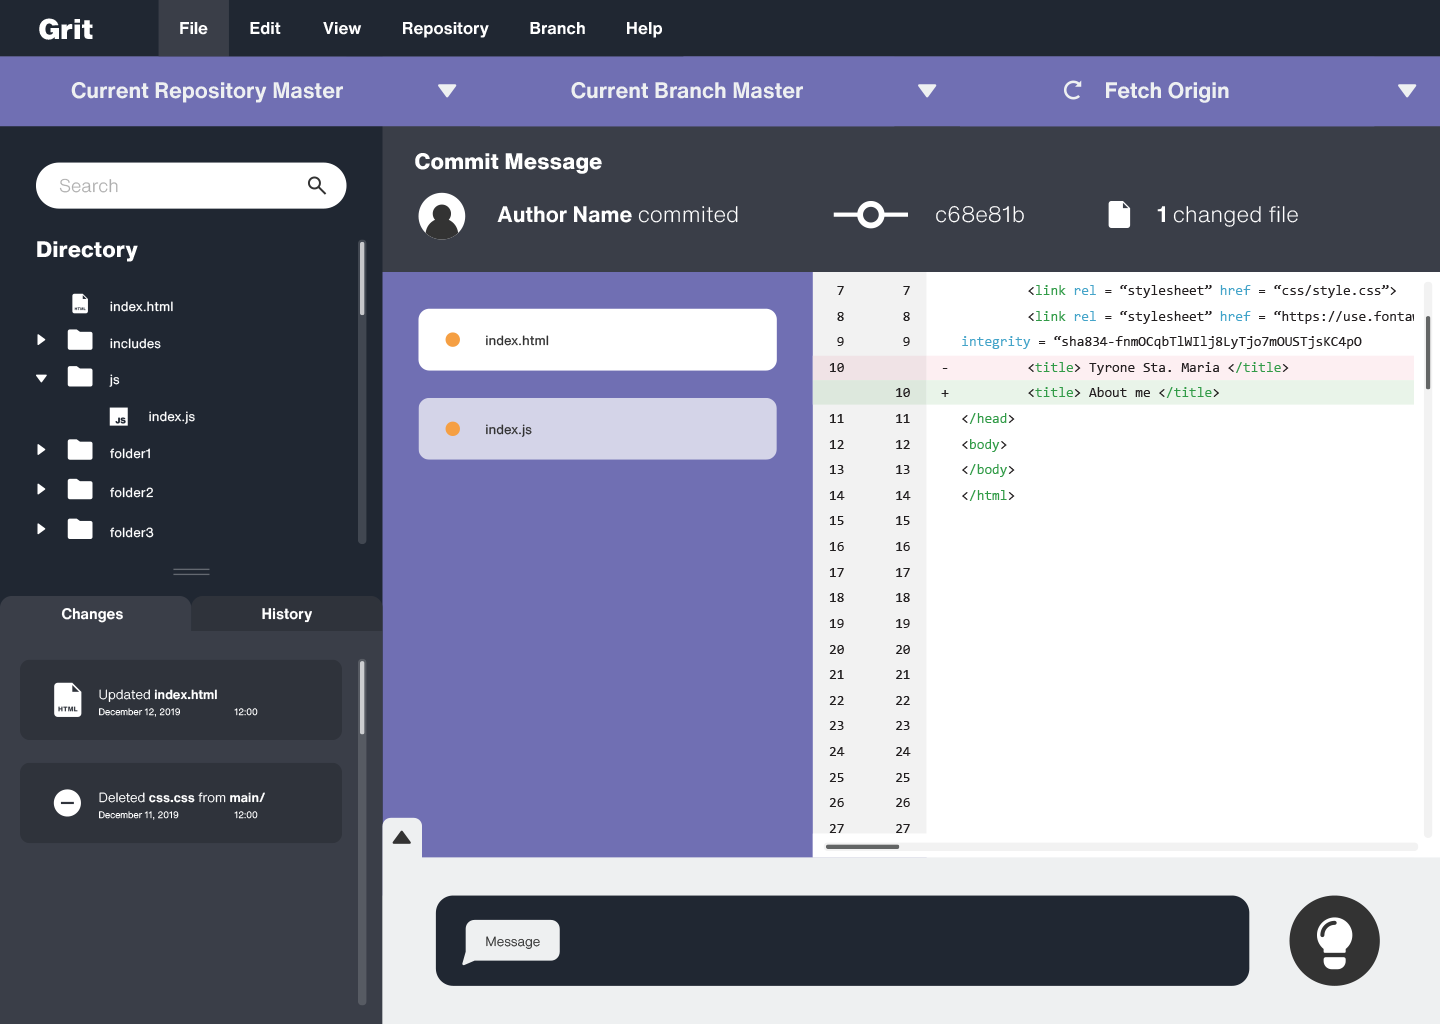
\includegraphics[scale=0.72]{figures/mockup1}
    \caption{caption here }
    \label{fig:mockup}
\end{figure}

\begin{figure}
    \centering
    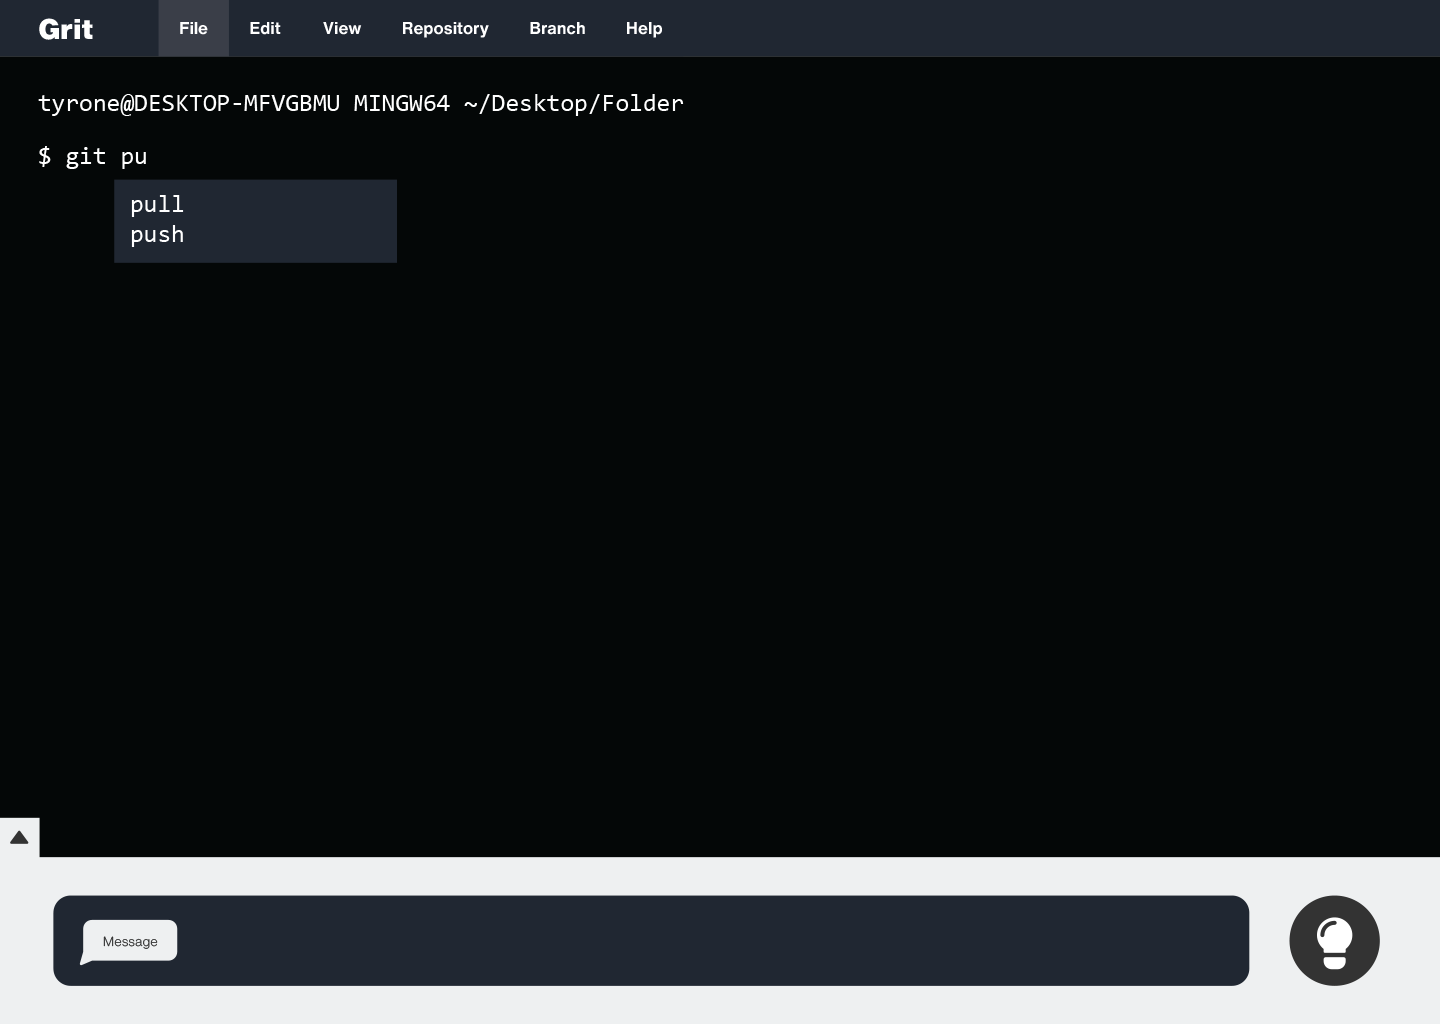
\includegraphics[scale=0.72]{figures/console1}
    \caption{caption here }
    \label{fig:console}
\end{figure}

Upon analyzing the data gathered, we designed a prototype that is intended to help novice programmers in integrating DevOps in their projects and processes. We name this proposed system as \textit{Grit}, which shall serve as a platform to guide novice programmers starting out with DevOps. It shall have the regular features from Git but will be augmented with 6 main features namely: (1) \texit{Version Control module}, (2) Virtual Assistant, (3) Command Line with Predictive Text, (4) Coachmarks, (5) Practice with Codeblocks and a feature accessed only thru online called (6) Find-a-Coach. 

See Fig. \ref{fig:mockup} to view these features. The Version control module is based from GitHub desktop which runs git commands such as pull, push, commit, and etc.The Virtual Assistant serves as guided walkthrough to the git commands and its functions. The Command line feature allows the users to call git commands with predictive text. The Coachmark enables first time users to navigate thru the system easily. The Practice with Codeblocks feature helps users to practice and understand the basic git commands. Lastly, the Find-a-Coach feature is an online mentoring tool that allows novices to find a mentor that will guide them in their DevOps process in real-time. With these proposed features, novices can be accustomed to the DevOps process but these can be verified thru further tests and experiments. 







\section{Limitation and Future Work}



\section{Conclusion}
hello


% \begin{table}
%   \centering
%   \begin{tabular}{l r r r}
%     % \toprule
%     & & \multicolumn{2}{c}{\small{\textbf{Test Conditions}}} \\
%     \cmidrule(r){3-4}
%     {\small\textit{Name}}
%     & {\small \textit{First}}
%       & {\small \textit{Second}}
%     & {\small \textit{Final}} \\
%     \midrule
%     Marsden & 223.0 & 44 & 432,321 \\
%     Nass & 22.2 & 16 & 234,333 \\
%     Borriello & 22.9 & 11 & 93,123 \\
%     Karat & 34.9 & 2200 & 103,322 \\
%     % \bottomrule
%   \end{tabular}
%   \caption{Table captions should be placed below the table. We
%     recommend table lines be 1 point, 25\% black. Minimize use of
%     table grid lines.}~\label{tab:table1}
% \end{table}



%



% BALANCE COLUMNS
\balance{}

% REFERENCES FORMAT
% References must be the same font size as other body text.
\bibliographystyle{SIGCHI-Reference-Format}
\bibliography{myreferences}

\end{document}

%%% Local Variables:
%%% mode: latex
%%% TeX-master: t
%%% End:

